% Ready-to-paste draft; figure/table paths are package-local and should be
% translated to the manuscript figure registry names at insertion time.
\subsection*{A2. Train/test overlap for FT-600K}

\noindent\textbf{Reviewer comment.}
\begin{quote}
\itshape
``Rule out train/test overlap for FT-600K: report the minimum SOAP-distance (or RMSD) between each in-gap NEB image and its nearest fine-tuning frame, or re-run FT-600K with the NEB-adjacent trajectory segment excluded, and confirm the 0.16 eV result survives.''
\end{quote}

\noindent\textbf{Response.}

We thank the reviewer for identifying this important provenance check. The
fine-tuning source for FT-600K consists of 600~K AIMD trajectories; NEB output,
NEB optimization frames, and NEB-adjacent path segments were not included in
the fine-tuning source. Thus the requested segment exclusion is already
satisfied at the source level rather than being imposed retrospectively after
the model was trained. We nevertheless performed the requested geometry-level
audit to test for close homologues between the target fixed-path images and
the declared grouped training files.

For the 25 retained five-image fixed-path structures from paths 1--2, 1--3,
1--4, 1--5, and 1--7, the full grouped FT-600K training file contains 1,786
frames and the Scratch-5\% control contains 89 frames. The minimum SOAP cosine
distances to any target image are $5.43\times10^{-4}$ and
$6.37\times10^{-4}$, respectively; the smallest comparable Cr-local RMSDs
are 2.06 and 2.06~\AA. No exact fingerprint match or near-duplicate match was
found under the declared audit gates (SOAP $\le 10^{-4}$ and RMSD $\le
0.05$~\AA). The RMSD comparison is reported only for composition-compatible
local environments; SOAP is the all-image audit.

The source-level exclusion and the direct near-duplicate audit answer literal
leakage. To place the result in the benchmark's task-conditioned framework, we
also assembled the distribution atlas in Fig.~\ref{fig:task_conditioned_atlas}.
The atlas deliberately separates the DFT/reference potential-energy surface
from the MLIP-generated potential-energy surface. The retained common
SOAP/PCA diagnostic contains 250 historical training, 122 validation, 124
test, and 25 fixed-path NEB structures. In this descriptive representation,
the held-out AIMD frames have a median nearest distance of approximately
0.01, whereas the fixed-path NEB images have a median distance of
approximately 213.74. This supports the interpretation that the NEB probe is
a distinct configuration-space direction, but it is not used as a calibrated
single-number OOD score.

The atlas also keeps equilibrium MD and failure/CAR trajectories on the MLIP
lane. In the 639-frame stage-balanced failure diagnostic, the median paired
force disagreement increases from 0.22~eV~\AA$^{-1}$ in the early-stable
window to 8.49~eV~\AA$^{-1}$ at the threshold window. This is a paired MLIP
disagreement diagnostic, not DFT error and not calibrated uncertainty. The
descriptor distance itself is not monotonic across the failure windows, so we
do not claim a universal scalar OOD ladder.

Finally, we repeated the FT-600K comparison under the trajectory-grouped split
using seeds 123, 234, and 345. On in-gap pathway 1--4, the grouped multi-seed
absolute fixed-path barrier error is $0.47\pm0.12$~eV for FT-600K,
$1.20\pm0.27$~eV for Scratch, and $0.68\pm0.20$~eV for Scratch-5\%; the
single-seed MPA0 comparator gives 0.24~eV. The historical 0.16~eV point
estimate is therefore not reproduced by the grouped multi-seed evaluation.
We report this directly rather than claiming that the historical value
survives. The conclusion is consequently task-conditioned model selection:
the absence of leakage is supported, while barrier fidelity must be assessed
separately from near-equilibrium RMSE and MD observables.

\noindent\textbf{Manuscript change.}

We added the source-level NEB exclusion and the SOAP/RMSD audit to Methods
Sec.~2.1 and the grouped in-gap results in Sec.~3.3.3. The task-conditioned
distribution atlas is cited in the Evaluation Framework and reproduced in the
SI with its source/status tables. The four task layers are static RMSE,
equilibrium/near-equilibrium MD, fixed-path versus self-relaxed NEB, and
failure/CAR trajectories. The figure caption states that fixed-path and
self-relaxed NEB are different operators, that provisional DFT candidates are
not final ground truth, and that MLIP-only disagreement is not DFT error.

\begin{figure*}[t]
\centering
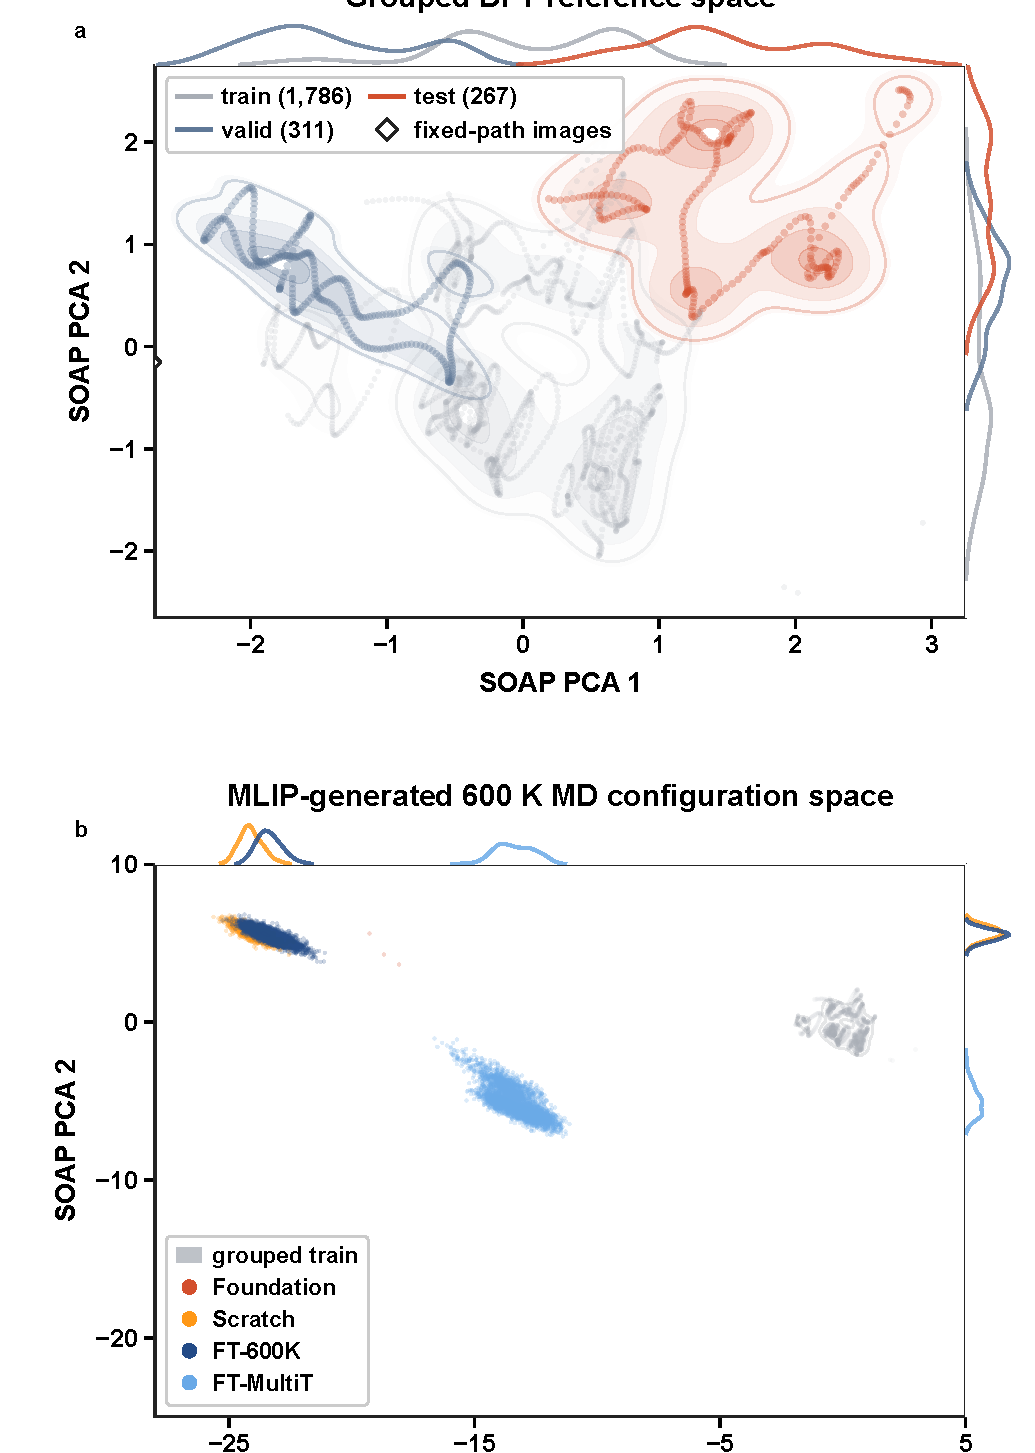
\includegraphics[width=\textwidth]{analysis/task_conditioned_distribution_atlas_20261018/figures/fig_task_conditioned_distribution_atlas.pdf}
\caption{\textbf{Task-conditioned distribution atlas across two potential-energy-surface lanes.} (a--d) DFT/reference-PES evidence for the static grouped reference split, held-out near-equilibrium AIMD frames, fixed-path NEB images, and four local-cell DFT recovery cases. The common SOAP/PCA panels use a retained historical fit for descriptive comparison. (e--h) MLIP-generated observables: grouped static RMSE, equilibrium-MD stability and seed spread, protocol-separated fixed-path/self-relaxed NEB errors, and failure/CAR force error with an MLIP-only committee-disagreement inset. JHU model colors are used only for model-family comparisons. Fixed-path and self-relaxed NEB are not pooled; provisional DFT path values and reconstructed local-cell DFT values remain explicitly status-labeled.}
\label{fig:task_conditioned_atlas}
\end{figure*}

